\documentclass[border=10pt]{standalone}

\usepackage{tikz}
\usepackage{tikzsymbols}
\usetikzlibrary{calc,patterns,shapes.geometric}

\def\centerarc[#1](#2)(#3:#4:#5){\draw[#1] ($(#2)+({#5*cos(#3)},{#5*sin(#3)})$) arc (#3:#4:#5);}

\begin{document}
	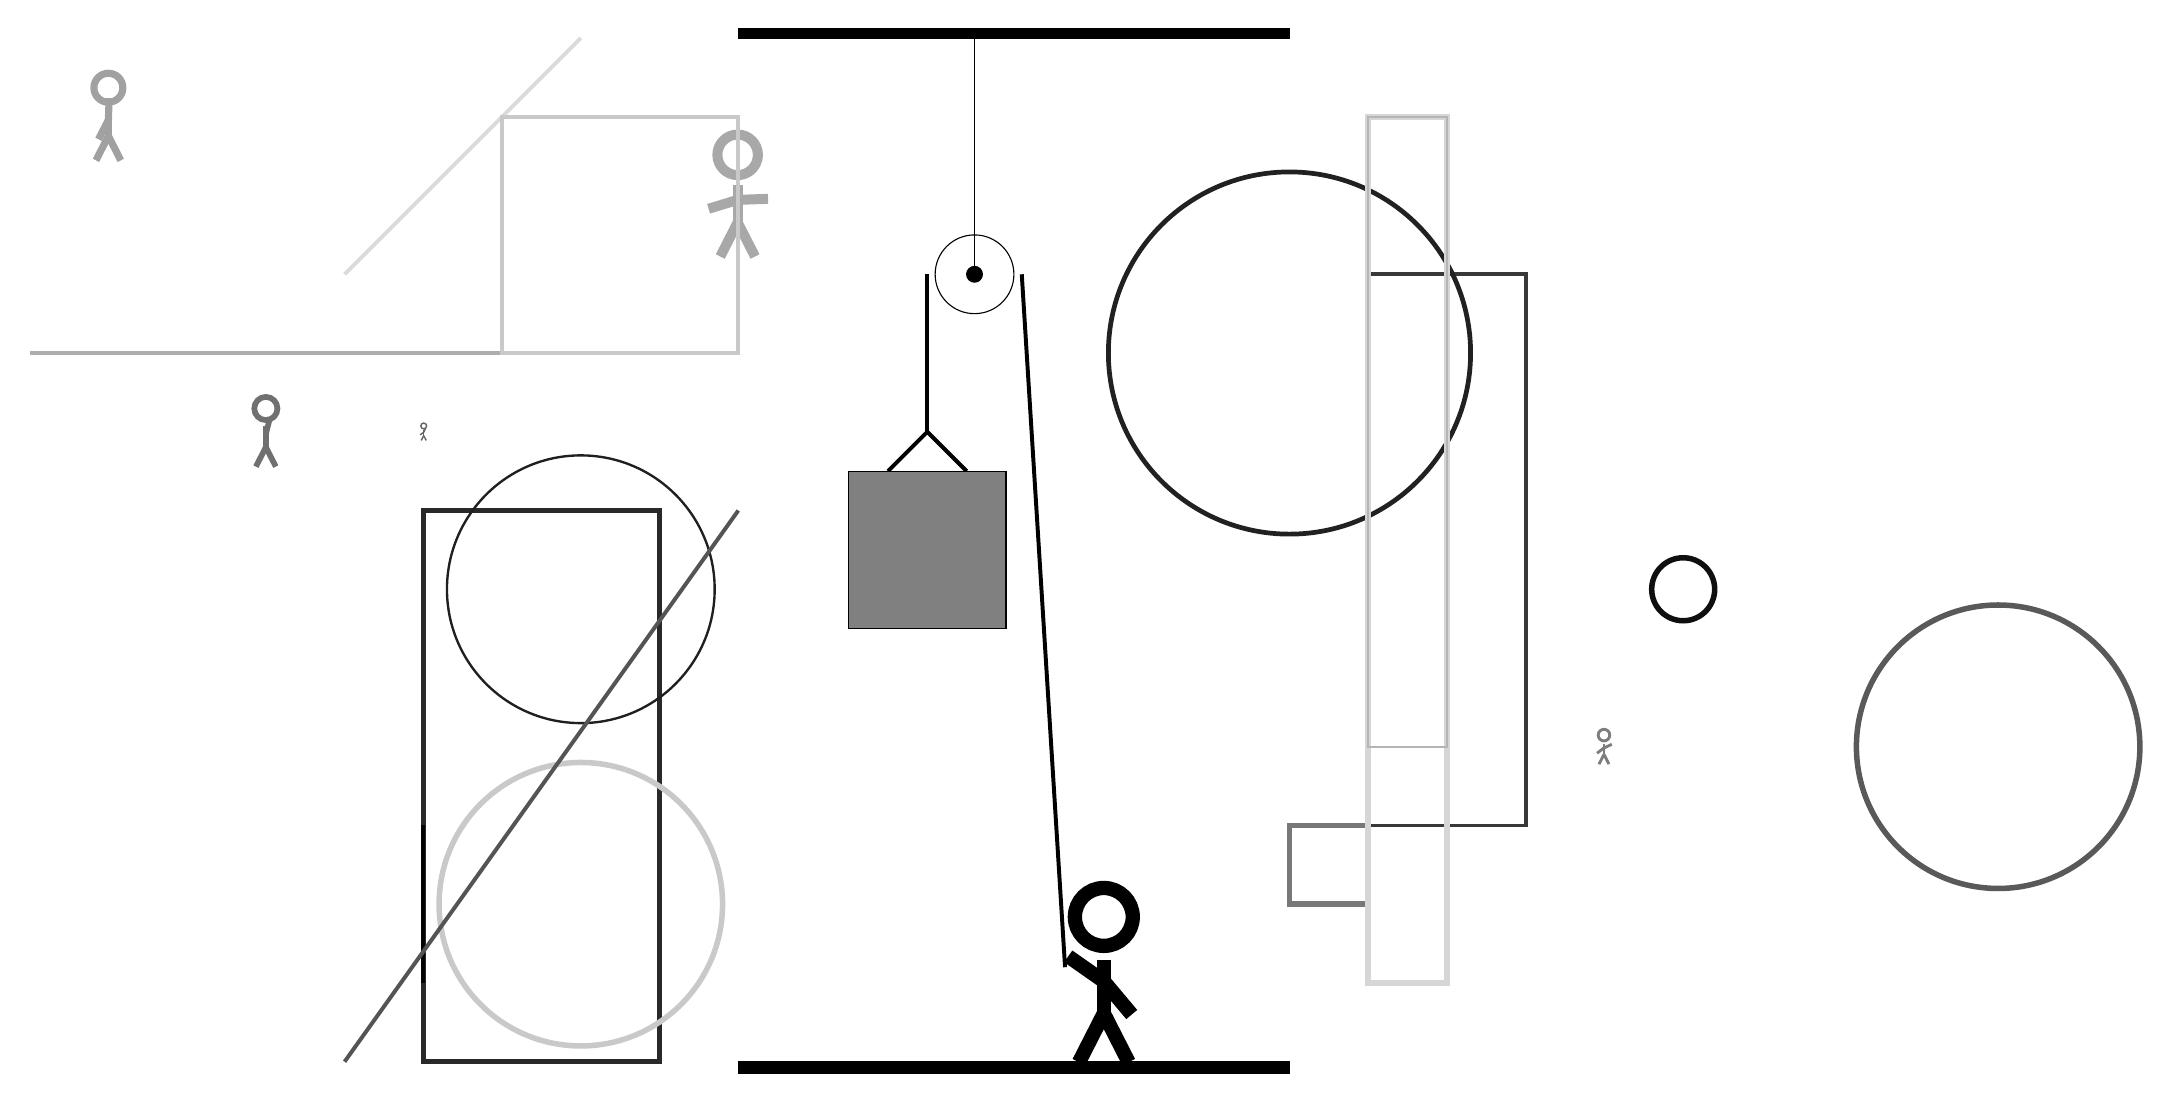
\begin{tikzpicture}
		%%%%% START %%%%%
		
		\draw[fill=black] (-2, 10) rectangle (5, 10.125);
		
		\draw (1, 7) circle (0.5);
		\draw[fill=black] (1, 7) circle (0.1);
		\draw (1, 10) -- (1, 7);
		
		\draw[line width=0.5mm] (-0.1, 4.5) -- (0.4, 5.0) -- (0.9, 4.5);
		\draw[fill=black!50] (-0.6, 4.5) rectangle (1.4, 2.5);
		
		\draw[line width=0.5mm] (0.4, 7) -- (0.4, 5.0);
		\centerarc[line width=0.5mm](1, 7)(0:180:0.6);
		\draw[line width=0.5mm](1.6, 7) -- (2.15, -1.8);
		
		\node at (2.6, -1.9) {\Strichmaxerl[10][-35][-50]};
		
		\draw[line width=0.7mm, color=black!84] (-3, -3) rectangle (-6, 4);
		
		\node[line width=0.6mm, color=black!34] at (-2, 8) {\Strichmaxerl[7][17][2]};
		\draw [line width=0.7mm, color=black!94](10, 3) circle (0.4);
		\draw [line width=0.7mm, color=black!65](14, 1) circle (1.8);
		\draw[line width=0.5mm, color=black!14](-7, 7) -- (-4, 10);
		\node[line width=0.5mm, color=black!51] at (9, 1) {\Strichmaxerl[2][37][25]};
		\draw [line width=0.3mm, color=black!88](-4, 3) circle (1.7);
		\node[line width=0.3mm, color=black!37] at (-10, 9) {\Strichmaxerl[5][63][88]};
		\draw[line width=0.5mm, color=black!78] (6, 0) rectangle (8, 7);
		\node[line width=0.5mm, color=black!56] at (-8, 5) {\Strichmaxerl[4][90][76]};
		
		\draw[line width=0.5mm, color=black!32](-4, 6) -- (-11, 6);
		\draw [line width=0.7mm, color=black!21](-4, -1) circle (1.8);
		\draw[line width=0.7mm, color=black!53] (6, -1) rectangle (5, 0);
		
		\draw [line width=0.6mm, color=black!87](5, 6) circle (2.3);
		\draw[line width=0.7mm, color=black!16] (6, 9) rectangle (7, -2);
		\node[line width=0.7mm, color=black!61] at (-6, 5) {\Strichmaxerl[1][33][66]};
		\draw[line width=0.5mm, color=black!99](-6, 0) -- (-6, -2);
		\draw[line width=0.5mm, color=black!21] (-2, 6) rectangle (-5, 9);
		\draw[line width=0.5mm, color=black!67](-7, -3) -- (-2, 4);
		
		\draw[line width=0.3mm, color=black!29] (6, 9) rectangle (7, 1);
		
		\draw[fill=black] (-2, -3) rectangle (5, -3.15);
		
		%%%%% END %%%%%
	\end{tikzpicture}
\end{document}